\documentclass[10pt,twocolumn,letterpaper]{article}
\usepackage[pagenumbers]{cvpr}
\usepackage{times}
\usepackage{graphicx}
\usepackage{booktabs}
\usepackage{microtype}
\usepackage{amsmath}
\definecolor{cvprblue}{rgb}{0.21,0.49,0.74}
\usepackage[pagebackref,breaklinks,colorlinks,allcolors=cvprblue]{hyperref}

\def\confName{Computer Vision Project}
\def\confYear{2026}
\title{Income-Related Performance Gaps in Vision-Language Models}
\author{Diya Tiwari \and Riya Katikar}

\begin{document}
\maketitle

\begin{abstract}
We study whether pretrained vision-language models perform differently on pictures of household objects from four income groups in Dollar Street. The benchmark contains 168 images from six categories, with seven images in every category-income cell. We compare CLIP, BLIP, Qwen2.5-VL, InternVL3.5, and YOLO-World without fine-tuning. CLIP classification and every automatic caption measure scored higher on the highest-income quartile than the lowest, while Qwen and InternVL classification changed little. A two-rater review showed that vocabulary matching understated BLIP caption quality. The measured gap depends on the model, task, and evaluation metric.
\end{abstract}

\section{Introduction}
The same household object can look different across homes. A stove may be built into a kitchen, placed on a table, or use solid fuel. Models trained largely on web image-text pairs may be more familiar with some forms than others. Earlier Dollar Street work found income-related differences in CLIP alignment and retrieval~\cite{nwatu2023}. We ask: \emph{How does performance on six household-object categories vary across four income quartiles when each category is equally represented?} Income groups the images; it is not treated as the cause of an error.

\section{Method}
\paragraph{Dataset.} We used the public 1,600-row Dollar Street test split~\cite{rojas2022}. Income records monthly consumption per adult equivalent in PPP-adjusted US dollars. After removing 45 multi-label rows, we formed quartiles from 1,555 eligible records. The evaluation subset has 168 images from 44 countries and six categories: roof, light source, stove, trash container, switch, and footwear. Each of the 24 category-quartile cells has seven images. This controls category frequency, although the subset is not representative of the population and regional counts remain unequal.

\paragraph{Models and tasks.} CLIP ViT-B/32~\cite{radford2021} performed six-way zero-shot classification with ``a photo of a \{label\}.'' BLIP-base~\cite{li2022} generated an unprompted caption and a caption beginning with the label-free prefix ``the main household object in this image is.'' Qwen2.5-VL-3B-Instruct~\cite{bai2025} and InternVL3.5-2B~\cite{wang2025} used the same forced-choice classification instruction and short, location-neutral caption instruction. YOLO-World-small-v2~\cite{cheng2024} received the six labels with a 0.25 confidence threshold. Dollar Street has no bounding boxes, so YOLO-World is reported as an image-level correct-class detection rate; mAP and IoU cannot be calculated.

CLIP used its 224-pixel checkpoint processor and BLIP its 384-pixel processor. Qwen used a 256-token visual budget, InternVL used $448\times448$ RGB inputs with ImageNet normalization, and YOLO-World used the Ultralytics pipeline. Generation was deterministic. The repository includes the manifest, identifiers, prompts, outputs, and run settings.

\paragraph{Evaluation.} Classification uses top-1 accuracy. Caption recall checks for a predefined category term or synonym using whole-term matching. Two raters independently reviewed all 336 BLIP captions for object correctness, non-informativeness, and hallucination, then resolved disagreements. We report raw agreement and Cohen's $\kappa$. A separate one-rater check used a fixed 84-image sample for Qwen captions. The main gap is Q4 minus Q1, with a 95\% category-stratified bootstrap interval from 2,000 resamples using seed 2026. We checked all 1,344 prediction rows for coverage, duplicate keys, and missing metrics.

\section{Results and analysis}
\begin{table}[t]
\caption{Scores (\%) by income quartile. Each quartile has 42 images. Metrics are task-specific and should not be compared as if they measured the same output.}
\label{tab:results}
\centering
\setlength{\tabcolsep}{2.4pt}
\small
\begin{tabular}{lrrrrr}
\toprule
Model and task & Q1 & Q2 & Q3 & Q4 & All \\
\midrule
CLIP classification & 76.2 & 81.0 & 95.2 & 92.9 & 86.3 \\
Qwen classification & 85.7 & 88.1 & 83.3 & 88.1 & 86.3 \\
InternVL classification & 88.1 & 92.9 & 78.6 & 88.1 & 86.9 \\
YOLO-World detection & 11.9 & 14.3 & 14.3 & 21.4 & 15.5 \\
BLIP caption, baseline & 28.6 & 52.4 & 54.8 & 76.2 & 53.0 \\
BLIP caption, prompted & 26.2 & 54.8 & 45.2 & 78.6 & 51.2 \\
Qwen caption & 35.7 & 64.3 & 71.4 & 81.0 & 63.1 \\
InternVL caption & 42.9 & 59.5 & 66.7 & 64.3 & 58.3 \\
\bottomrule
\end{tabular}
\end{table}

\begin{figure}[t]
\centering
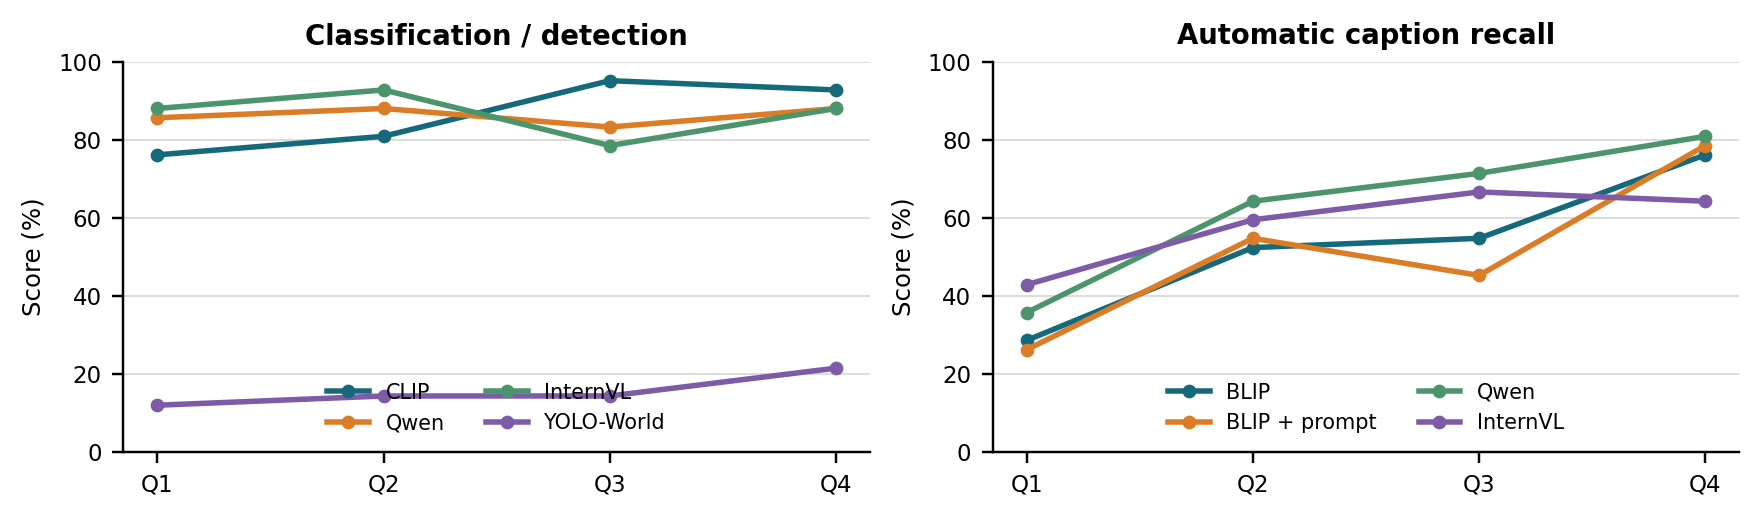
\includegraphics[width=\linewidth]{../assets/combined/scores_by_income.png}
\caption{Performance by income quartile. Caption recall shows a larger Q4--Q1 spread than classification; the plotted values match Table~\ref{tab:results}.}
\label{fig:income}
\end{figure}

The classifiers had similar overall accuracy (86.3--86.9\%), but their quartile results differed (Table~\ref{tab:results}). CLIP's Q4--Q1 gap was 16.7 points (95\% CI 2.4 to 28.6). The intervals for Qwen's 2.4-point gap ($-7.1$ to 14.3) and InternVL's zero-point gap ($-9.5$ to 9.5) included zero. Thus, the CLIP pattern did not appear in both instruction-following classifiers.

Automatic caption recall was higher in Q4 than Q1 for every caption condition. The gaps were 47.6 points for unprompted BLIP, 52.4 for prompted BLIP, 45.2 for Qwen, and 21.4 for InternVL. Manual review gave a different view of BLIP. Object correctness was 80.4\% without the prompt and 83.9\% with it, compared with automatic recall of 53.0\% and 51.2\%. The prompt reduced automatic recall by 1.8 points, but improved human-rated correctness by 3.6 points and reduced hallucinations from 16.7\% to 12.5\%. Agreement was 89.3\% ($\kappa=0.65$) for object correctness and 94.0\% ($\kappa=0.77$) for hallucination. In the separate Qwen sample, automatic recall was 57.1\% and clear semantic recall was 70.2\%; 11 of 84 captions remained uncertain. The term list missed reasonable descriptions such as \emph{bucket} or \emph{basket} for a trash container.

Category results showed different weaknesses. CLIP was weakest on light sources (60.7\%); Qwen and InternVL were weakest on roofs (39.3\% and 50.0\%). YOLO-World found 57.1\% of footwear and 25.0\% of stoves, but none of the roofs, light sources, or switches. In one failure case, CLIP labelled a small red fuel can as a stove while BLIP described the visible can. In another, a roof occupied little of the frame and was classified as a light source. These cases explain why we include category results and manual caption review.

\section{Discussion and limitations}
The results do not support one common income pattern across all models. CLIP and the automatic caption measures favored Q4, whereas Qwen and InternVL classification were nearly flat. The BLIP comparison also depended on the metric because term recall missed wording that raters accepted.

The study covers 168 selected images and six categories. Balancing removes category-frequency differences but does not control country, region, image quality, scene complexity, or variation within a category. Quartiles are defined within the test split, and the intervals describe this benchmark only. Models never received income information, so the results show an association and do not establish that income caused errors. The Gradio interface demonstrates the five models on uploaded images; it is not a second evaluation dataset.

\section{Related work}
Dollar Street provides household-object images with country, region, and income metadata~\cite{rojas2022}. Nwatu et al. evaluated CLIP alignment and prompt-based retrieval across income groups~\cite{nwatu2023}. We use a category-balanced subset, test six-way recognition and captioning, and compare five model families on the same images. CLIP links the experiment to earlier work~\cite{radford2021}, while BLIP adds caption generation~\cite{li2022}. Qwen2.5-VL and InternVL3.5 add instruction-following VLMs~\cite{bai2025,wang2025}, and YOLO-World adds open-vocabulary detection~\cite{cheng2024}. A gap observed with one model or automatic metric did not always carry over to another.

{\small
\bibliographystyle{ieeenat_fullname}
\bibliography{main}
}
\end{document}
